In this section we apply the techniques covered in the previous sections to a real world use case.
\subsection{Problem statement}
We want to apply symbolic regression on the output of a simulator. The simulator we use for our experiment is a high performance tool \citep{stride} that models the spread of infectious diseases. 
A single simulation instance is computationally expensive. We would like to construct a surrogate model that approximates the simulator. A surrogate model can offer insights into the underlying process that the resulting data cannot. Symbolic regression offers a white box model in addition to this advantage. We can use symbolic regression to obtain such a model, but in order to do so we need to obtain input and output data. 
Generating all simulation output in sequence leads to significant downtime for the practitioner. Using our incremental support detailed in section \ref{subsec:incremental} we offer the practitioner partial results during this downtime. These results can be used by a domain expert to modify the design of experiment instead of having to wait until the entire process has completed. Our tool is able to reuse the partial results as seeds for new runs. We will investigate if this approach can lead to an improved model.
The value for the practitioner in this approach is twofold : incremental informative results are offered during an otherwise inactive time allowing for a feedback loop with the simulator, and a possible improvement in the final model can be obtained by seeding our regression tool.
\paragraph{Design of experiment}
Combining all possible values for all parameters is infeasible. 
Given the size of the parameter space of the simulator a Design Of Experiment (DOE) is constructed where the coverage of the parameter space is maximized while minimizing the number of combinations for all parameters. 

We would like to have a space filling design that maximizes the sampling of the parameter space while minimizing the number of evaluation points.
In this experiment we apply a Latin Hypercube Design (LHD). 
Given k dimensions (parameters) and a desired output set of p points, we have that 
\[
p_i = (p_{i0}, ..., p_{i k-1}) \in (0, p -1)^k
\]
with for each dimension j all $p_{ij}$ are distinct. This avoids a full factorial combination, while still covering the entire parameter space. 
The idea behind a LHD is that it avoids collapsing. Suppose we have j parameters that have little or no effect on the output. If we construct a space filling design based on sampling alone all points $p_{ij}$ will evaluate to the same output value (minus noise) for all j. In other words, we execute j evaluations without gaining information about the underlying model. By virtue of the problem statement we do not know the effect a parameter has on the output. A LHD avoids collapsing by using the constraint that no two points share coordinate values. A side effect of this is that if we reduce a d-dimensional LHD to a d-i dimensional LHD by simply removing the i dimensions from the design, the resulting design still forms a good space filling design.
Constructing such a LHD can be done in a variety of ways, typically using a distance measure linked to some concept of optimality. An often used measure is the euclidean distance measure :
\[
d(p_i, p_j) = \sqrt{\sum_{l=0}^{d-1}(p_{il}-p_{jl})^2}
\]
This distance measure is used to obtain a maximin LHD where
\[
min_{i \neq j} d(p_i,p_j)
\]
is maximal for all LHDs of size p. The maximin LHD is the most often used LHD in practice. In this work we will use the Audze-Eglais \citep{AudzeEglais, AudzeEglais2, AudzeEglais3} (AE) LHD, which uses the Euclidean distance measure but in addition obtains a uniform distribution of the individual points. 
The AE LHD is based on the concept of potential energy between design points, a measure based on the inverse of the euclidean distance.
\[
E^{AE} = \sum_{i=0}^{p-1} {\sum_{j=i+1}^{p-1} {\frac{1}{d_{ij}}}}
\]
The potential energy measure is minized in AE.
\paragraph{Interaction with regression tool}
We would like to obtain symbolic expressions relating parameters values to simulator output. These expressions can be used to gain insight into which parameters are correlated, which have a larger effect on output and which are irrelevant. 
We then execute the simulator on each configuration. With the execution of a single configuraton independent of all others this is an embarrassingly parallel problem. We combine the output of all configurations and feed them into our tool where we can apply symbolic regression or another machine learning technique in order to extract a model that approximates the simulator. The problem with this approach is twofold. We have to wait until the simulator has completed all configurations, then the SR tool executes on a large dataset. It has no known starting point so effectively performs a blind search in a huge search space. We can avoid both issues by using partial results from the simulator as input for the SR tool. The results from these partial samples ideally will provide a good starting point for the incrementally growing dataset. This last assumption only holds if the sequence of completed configurations is a good sample of the full dataset. We can enforce this by ordering the configurations but this is non trivial. Configurations will not have the same computational load for all simulations. Consider for example the population parameter in an epidemiological simulator. An increase in runtime for all configurations is expected if we increase this parameter. Simulating real world processes quickly leads to simulation runs that require significant computation time and resources to complete a single configuration. As an example an epidemiological simulator modelling the US population \cite{FRED} requires 4 hours on a supercomputer. The effect of changing a simulation parameter on the runtime of the simulator is domain specific.
Even if we take this into account in our scheduling, the parallel execution of any number of tasks is never deterministic. The order of configurations is not only important to avoid a bias for the full design, which would lead to overfitting. The initialization problem detailed in section \ref{subsubinvalidexpressions} reappears here. If the initial partial set of configurations is biased the probability is quite high that the resulting solutions are invalid expressions for the complete data set. When the ratio between known and unknown data is too large the probability increases that expressions are evolved that have a domain that does not include the unknown data.

\subsubsection{Experiment}
Epidemiological simulation is a vital tool for policy makers. Simply observing the real world process is a measure of last resort at unacceptable cost in human suffering, and the resulting data is not strictly predictive for new outbreaks. A single outbreak is a sample of a very large configuration space. The focus in policy making lies on prevention and insight, and for these aims simulation and surrogate modelling are essential. A theoretical model cannot approximate within a reasonable error margin the complexity of a real world process, while simulation, with a configurable set of parameters mimicking the real world process, can.
The simulator is configured to model a measles outbreak in a population of 5e5 in the city of Antwerp, Belgium. With immunization for this disease a concern worldwide we would like to obtain a surrogate model that can offer policy makers insights leading to preventative measures. Of vital importance here is the immunization aspect. Our research question for this case is : How does the immunization fraction influence the outbreak of measles ?
We investigate this use case within the context of this work, that is, we focus on the convergence characteristics of the process evolving the model rather than the domain specific implications of the surrogate model itself. We are interested in the value of the surrogate model at an intermediary stage in the process. How closely does this model exhibit the same trends as the underlying process? This relation in vital in order to justify our usage of partial results in the feedback loop between practitioner, simulator and regression tool.
\paragraph{Simulator configuration}
We construct a DOE with 3 dimensions, 30 points in total using the tool introduced in the work of \citep{DOE}. 
The following are the parameters used:
\begin{itemize}
\item Basic reproduction number (R0) : the number of persons an infected person will infect, [12-20]
\item Starting set of infected persons (S) : Number of persons in the population that is an infected person at the start of the simulation, [1-500]
\item Immunity fraction (I) : Fraction of the population that is immune to the disease. [0.75, 0.95]
\end{itemize}
The output parameter represents the attack rate, measured as the rate of new cases in the population at risk versus the size of the population at risk.
For each parameter we obtain 30 points uniformly chosen in their range. These are then combined in the DOE.
The simulator is run once for each configuration. 
\paragraph{Symbolic regression configuration}
\begin{itemize}
\item i: initial depth : 3
\item m: maximum depth : 6
\item p: population : 20
\item g: generations per phase : 60
\item f: phases : 30
\item archiving strategy : 4 best per phase
\item d: datapoints : 10, 20, 30
\end{itemize}
The total cost in fitness evaluations is then given by: 20*60*30*d.
We compare 3 approaches. First we run the CSRM tool on the entire dataset. This is the classical approach, the tool is not seeded and so starts a blind search. In a real world setting this would mean waiting until the simulator has run all 30 configurations.
In our second approach we split the data into incremental sections. After 10 configurations have completed we start the tool on this dataset. 
The best 4 results are saved to disk, then we run the tool with the result of 20 configurations and use the results from the previous run as a seed. The overlap between the two datasets will influence the effects of the initialization problem. Finally we use the results of the 20-point dataset as a seed for the 30 point run. 
The cost of running the 10 and 20 point runs to use as seed for the 30 point run is similar to the cost of the 30 point run. 
To ground the comparison our last approach runs the tool on the data from 30 configurations with double the amount of phases. This means that it has approximately the same number of fitness evaluations as the 10-20-30 combination. We compare all three to see which gains are made and at what cost.
We then compare the incremental technique without constant optimization in sequential mode in order to isolate the effect of reseeding the tool.
Then we apply the optimizers and run the experiment distributed to observe the change in convergence characteristics.
\subsection{Results}
\subsubsection{Fitness improvement}
We compare both seeded runs and the extended run with the normal 30-point run. In Figure \ref{fig:incrementalgain} we see that the fitness is improved by using the best results of the previous run on a partial data set. We have deliberately split our data set in such a was as to expose a risk here. If we run the tool with 20 datapoints seeded by a run of 10 datapoints, we see that the validated fitness actually decreases compared to a non seeded run. The ratio between new and known data is too large, leading to overfitting. If we seed the best results from the 20-point run into a 30 point configuration we see that both the training and validated fitness values significantly improve. 
The 30 point run with 60 phases has the same computational cost as the 10-20-30 runs combined, but gains little to nothing in convergence. We see that convergence is slowing, with training fitness improving by a factor of 1.1, but validation fitness worsens. This is a typical example of overfitting. The combined 10-20-30 run increases validation fitness with a factor of 1.13.
\begin{figure}
    \centering
    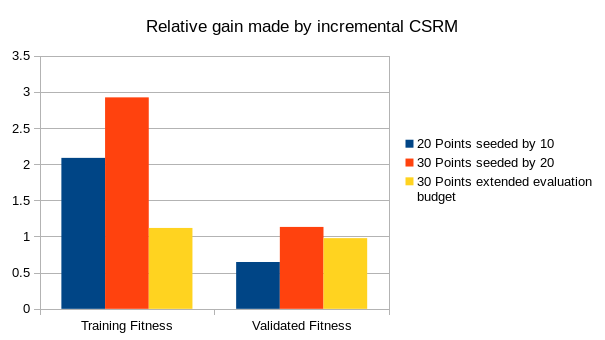
\includegraphics[width=\textwidth,height=\textheight,keepaspectratio]{figures/incrementalgain.png}
    \caption{Incremental fitness gain in CSRM.}
    \label{fig:incrementalgain}
\end{figure}
\subsubsection{Convergence behavior}
\paragraph{Fitness distribution}
In Figures \ref{fig:incrementalseededconvergence},\ref{fig:incrementalconvergence},\ref{fig:incrementaldoubleconvergence} we see how the convergence process evolves over time. 
Note the clustering patterns in the incremental runs. When seeded with solutions of previous runs we introduce information that the algorithm otherwise would have to discover. These seeds have fitness values somewhere between the randomly generated and optimal samples. Applying operators on them leads to a niching effect visualized in the fitness distribution. Seeding will not guarantee this effect, it is a possibility depending on how the seeds fit in the trajectory in the search space that the algorithm generates during its execution.
If we compare the fitness plots we clearly see that the seeded process has a different distribution compared to the unseeded runs. Around generation 1000 the convergence rate slows. Doubling the phases has little effect on the fitness distribution. 
\paragraph{Operator effectiveness}
In the plots we see the operator success rate and operator gains visualized. The first is the ratio between the number of applications of an operator that lead to improvement in fitness versus the total number of applications. The trendline is obtained by a cubic fit. This gives us an indication whether an operator is still effective, in particular it gives us the fraction of the population that is improved each generation by the operator. The second plot is the mean gain of an operator, it reflects how much the fitness of each generation is improved by an operator. The distinction is important, if fitness is improved by very small amounts the success rate will be high but the gain low. These statistics offer an insight into the convergence characteristics over generations. Instead of relying only on the end result we can directly observe the effects of the operators. For our comparison we see that there is little difference in gain or success rate between the three runs.
\paragraph{Constant folding}
The percentage of nodes saved is similar for all three runs. The plots show that constant subtrees are introduced at a constant rate and folded at the end of each generation. The savings plotted also give an indication of the incremental increase in nodes that could take place if folding was not implemented. 
 \begin{figure}
    \begin{subfigure}{0.6\textwidth}
        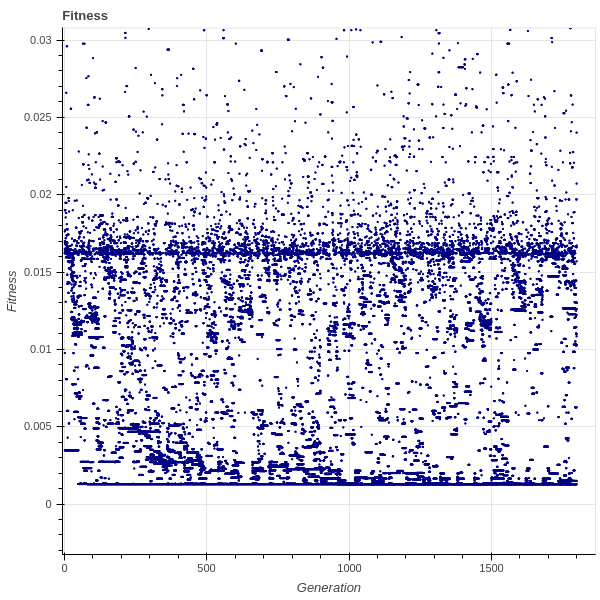
\includegraphics[width=0.8\linewidth]{figures/incrementalfitness30s.png}
        \caption{Fitness.}
    \end{subfigure}
    \begin{subfigure}{0.6\textwidth}
        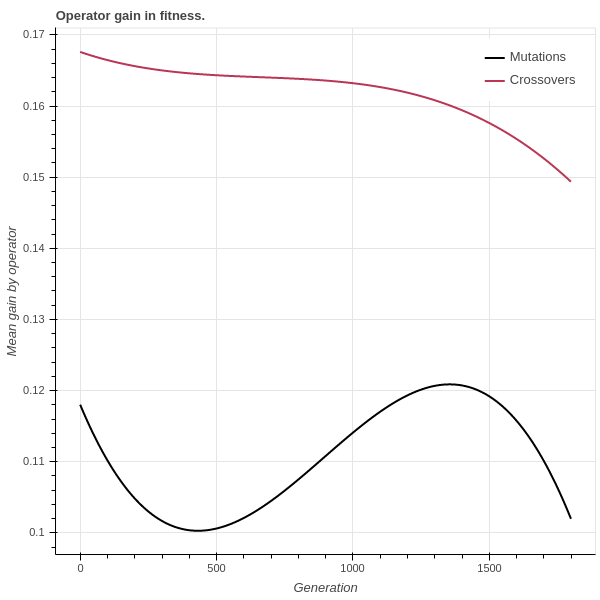
\includegraphics[width=0.8\linewidth]{figures/incrementaloperatorgain30s.png}
        \caption{Operator gain.}
    \end{subfigure}
        \begin{subfigure}{0.6\textwidth}
        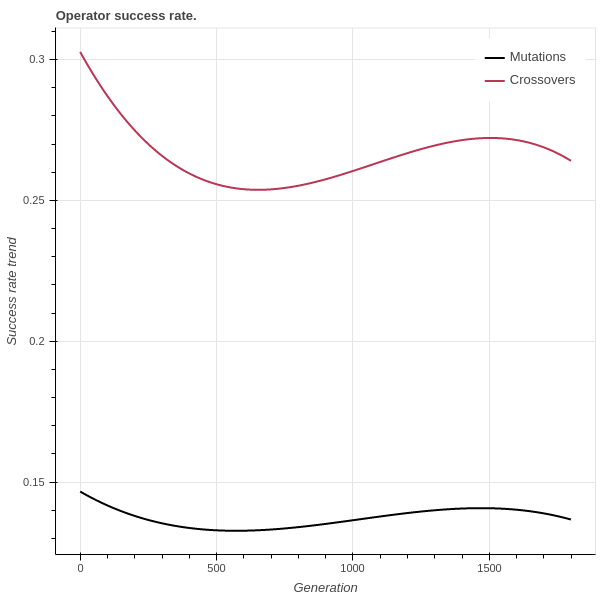
\includegraphics[width=0.8\linewidth]{figures/incrementaloperatorsuccessrate30s.png}
        \caption{Operator success rate.}
    \end{subfigure}
    \begin{subfigure}{0.6\textwidth}
        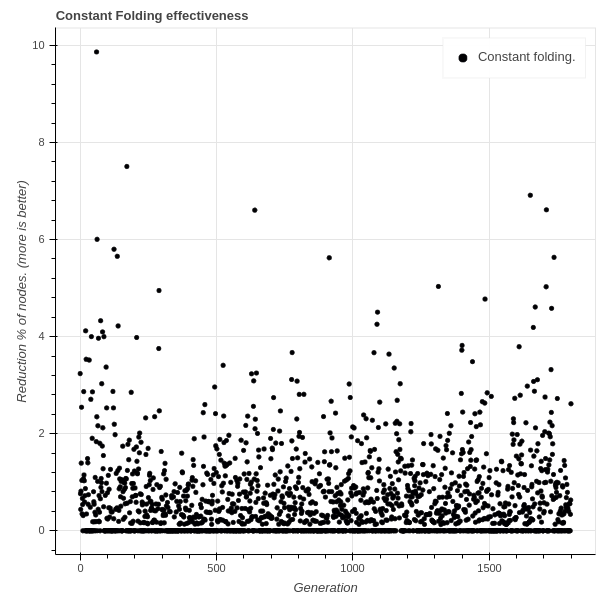
\includegraphics[width=0.8\linewidth]{figures/incrementalconstfolding30s.png}
        \caption{Constant folding savings.}
    \end{subfigure}
    \caption{Convergence behavior of incremental symbolic regression with 10-20-30 split.}
    \label{fig:incrementalseededconvergence}
\end{figure}
 \begin{figure}
    \begin{subfigure}{0.6\textwidth}
        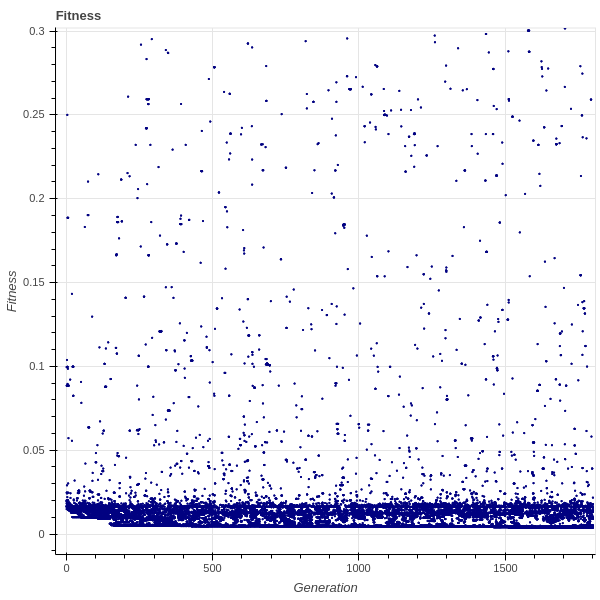
\includegraphics[width=0.8\linewidth]{figures/incrementalfitness30.png}
        \caption{Fitness.}
    \end{subfigure}
    \begin{subfigure}{0.6\textwidth}
        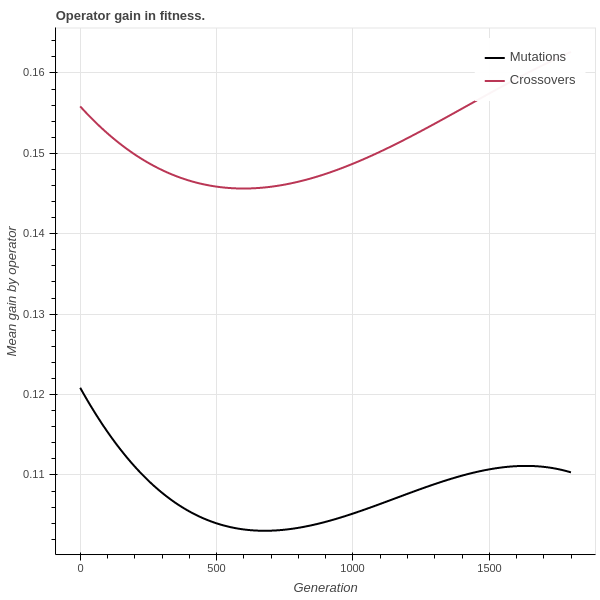
\includegraphics[width=0.8\linewidth]{figures/incrementaloperatorgain30.png}
        \caption{Operator gain.}
    \end{subfigure}
        \begin{subfigure}{0.6\textwidth}
        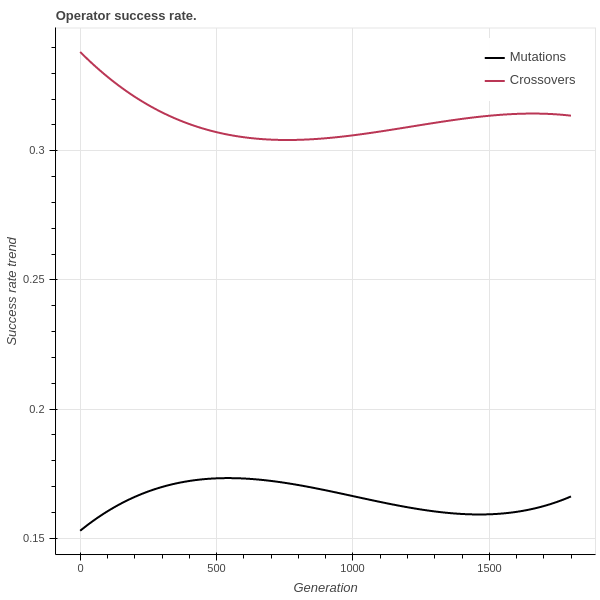
\includegraphics[width=0.8\linewidth]{figures/incrementaloperatorsuccessrate30.png}
        \caption{Operator success rate.}
    \end{subfigure}
    \begin{subfigure}{0.6\textwidth}
        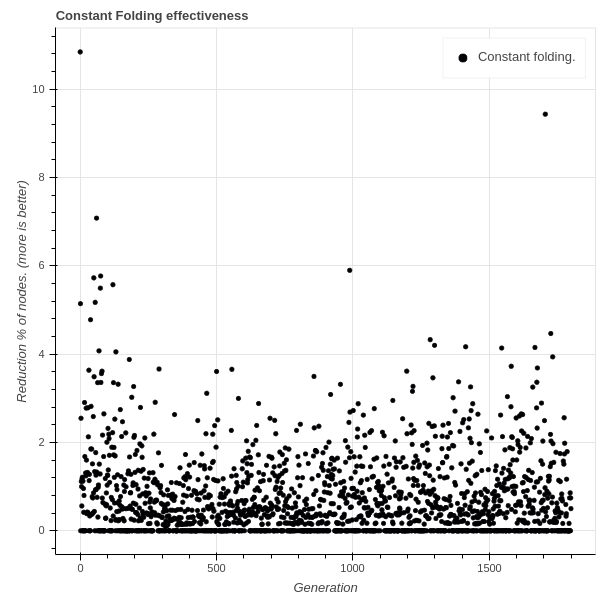
\includegraphics[width=0.8\linewidth]{figures/incrementalconstfolding30.png}
        \caption{Constant folding savings.}
    \end{subfigure}
    \caption{Convergence behavior of incremental symbolic regression without split.}
    \label{fig:incrementalconvergence}
\end{figure}
% [bcardoen@localhost src]$ python3 -m gp.paralleldriver -c 1 -t none -g 60 -p 20 -f 60 -x doe/input.csv -y doe/output.csv -m 6 -v -d 30 -q 3 -i 3

 \begin{figure}
    \begin{subfigure}{0.6\textwidth}
        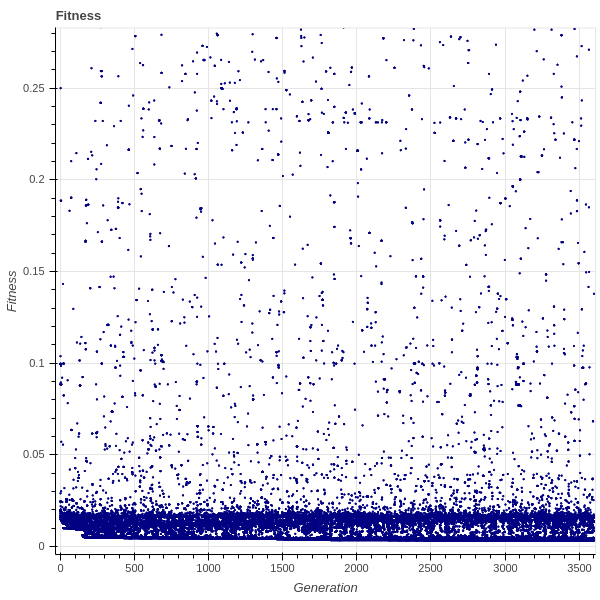
\includegraphics[width=0.8\linewidth]{figures/incrementalfitness30d.png}
        \caption{Fitness.}
    \end{subfigure}
    \begin{subfigure}{0.6\textwidth}
        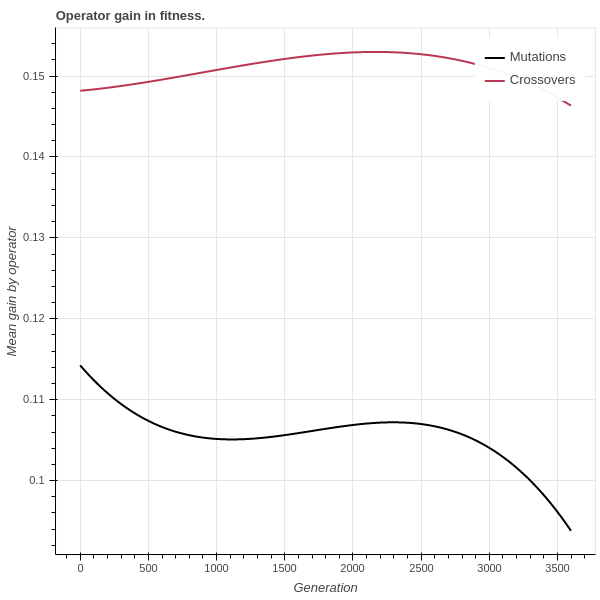
\includegraphics[width=0.8\linewidth]{figures/incrementaloperatorgain30d.png}
        \caption{Operator gain.}
    \end{subfigure}
        \begin{subfigure}{0.6\textwidth}
        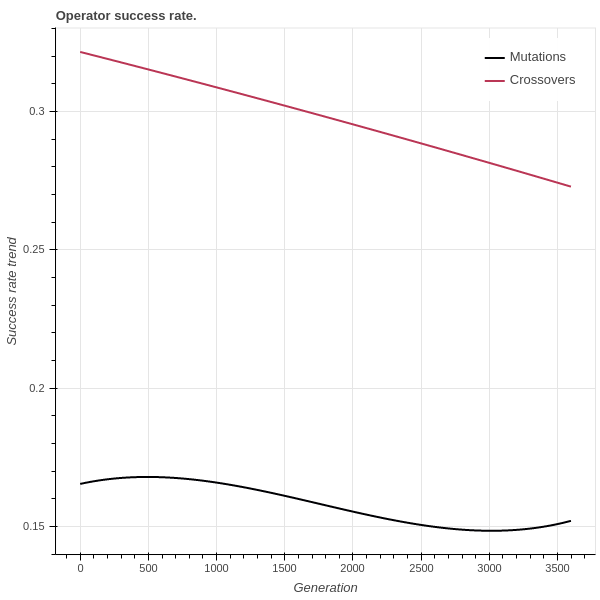
\includegraphics[width=0.8\linewidth]{figures/incrementaloperatorsuccessrate30d.png}
        \caption{Operator success rate.}
    \end{subfigure}
    \begin{subfigure}{0.6\textwidth}
        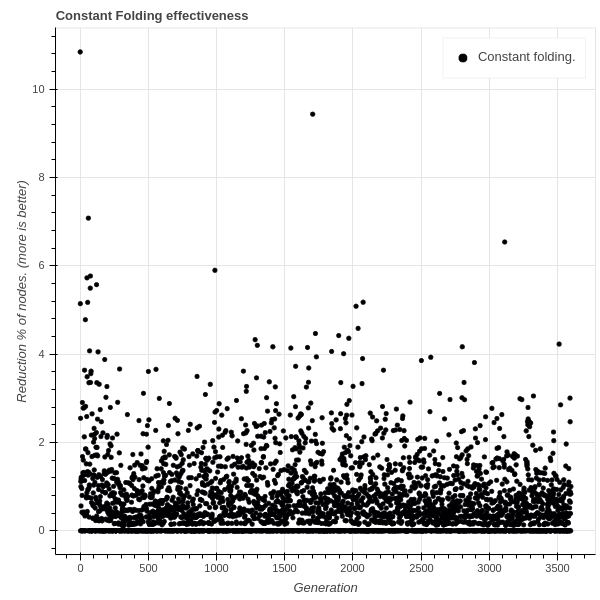
\includegraphics[width=0.8\linewidth]{figures/incrementalconstfolding30d.png}
        \caption{Constant folding savings.}
    \end{subfigure}
    \caption{Convergence behavior of incremental symbolic regression with identical computational cost as 10-20-30 split.}
    \label{fig:incrementaldoubleconvergence}
\end{figure}
\subsubsection{Optimizers}
We apply each of the three optimizers in a small run with the best results of the incremental approach as a seed. From our previous discussion we known that using a configuration with 30 phases is likely to result in overfitting. We use the results of the incremental 10/20/30 run as a seed and observe the convergence characteristics of applying the optimizers.
We would like to observe the effect of the optimizers in a seeded configuration. We focus on the best expression, and no longer the mean of the (sub)population. While the distribution of the fitness values as a measure is informative, it is of little worth to the practitioner who will be result oriented when applying a regression tool.
\paragraph{Configuration}
\begin{itemize}
\item i: initial depth : 3
\item m: maximum depth : 6
\item p: population : 20
\item g: generations per phase : 60
\item f: phases 2
\item archiving strategy : 4 best per phase
\item d: datapoints : 30
\item optimizer : ABC, PSO, DE, None
\item seeds : 4 best solutions from incremental 10/20/30 run
\end{itemize}
In order to isolate the optimizer gain we keep the total number of generations small in comparison to the 10/20/30 run (120 vs 3600).
\paragraph{Results}
In Figure \ref{fig:usecaseoptimizers} we see that the optimizers cannot improve the fitness value much beyond the seeded value. We see that even though fitness on the training data tends to increase, overfitting increases as well. ABC and PSO introduce overfitting. Interestingly enough DE results in a lower training fitness value compared to a run without optimizer, but has better validated fitness results. The expression with the best fitness value on training data is not necessarily the expression with the best fitness value on the validation data. Although we would like to have a strong correlation between the two, this is not always the case. This is one possible reason for the results shown. Note that the optimizers operate twice on the 4 best expressions. We see the same behavior observed in the benchmarks, the optimizers can easily introduce overfitting. A seeded configuration is especially sensitive to this behavior.
\begin{figure}
    \centering
    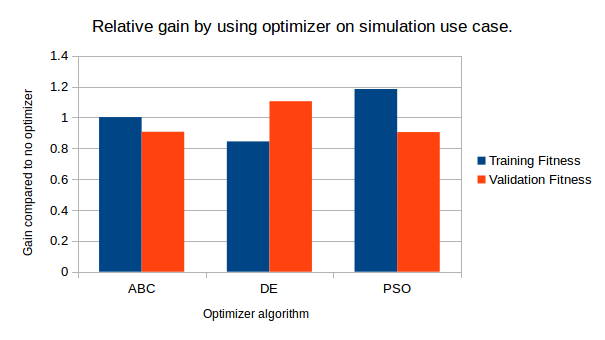
\includegraphics[width=\textwidth,height=\textheight,keepaspectratio]{figures/usecaseoptimizers.png}
    \caption{Optimizers applied to use case.}
    \label{fig:usecaseoptimizers}
\end{figure}

\subsubsection{Distributed}
We seed a distributed run with the results of the 10/20/30 run and compare the topologies in terms of fitness improvement and speedup.
\paragraph{Configuration}
\begin{itemize}
\item i: initial depth : 3
\item m: maximum depth : 6
\item p: population : 20
\item g: generations per phase : 60
\item f: phases 30
\item archiving strategy : 4 best per phase
\item d: datapoints : 30
\item optimizer : None
\item seeds : 4 best solutions from incremental 10/20/30 run
\item topology : Tree, Grid, RandomStatic, Disconnected
\item number of processes : 25
\end{itemize}
\paragraph{Results}
In Figure \ref{fig:usecasedistributed} we compare the gain in fitness on the validation data for the tree, grid and randomstatic topologies compared to the disconnected topology. We can clearly see that the diffusion in the grid topology leads to the highest gain, followed by the tree topology. Interestingly enough, the random topology scored worse than the disconnected topology. This can occur when a local optimum is communicated early to the other processes which then dominates the remainder of the process. The effect on the runtime is measured in Figure \ref{fig:usecasespeedup}. We see that the tree topology has minimal overhead and runs nearly as fast as the disconnected topology where no synchronization or communication overhead is present. The grid topology suffers a 2x performance penalty and the random topology finds the middle ground between the two. During the experiment we observed that the processes in the tree and disconnected topologies varied as much as 4 phases. This is what we expected, in this tree topology the distance between two processes is at most 4 (depth of a 25-node binary tree). This is an important observation, if we increase the number of processes the tree topology will actually scale better. The delay tolerance allows the tree topology this scaling effect.
\begin{figure}
    \centering
    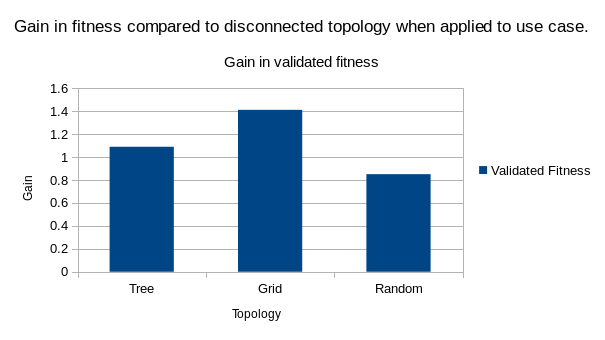
\includegraphics[width=\textwidth,height=\textheight,keepaspectratio]{figures/usecasedistributed.png}
    \caption{Incremental distributed CSRM applied to use case.}
    \label{fig:usecasedistributed}
\end{figure}
\begin{figure}
    \centering
    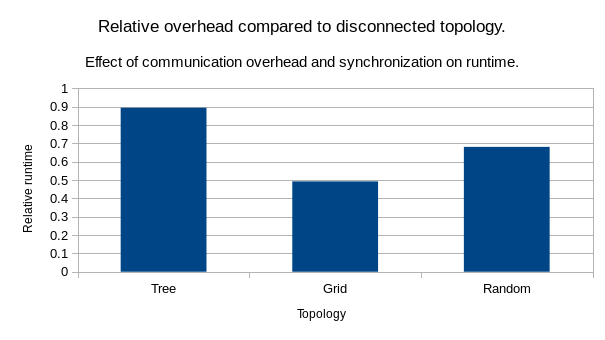
\includegraphics[width=\textwidth,height=\textheight,keepaspectratio]{figures/usecasespeedup.png}
    \caption{Runtime impact of synchronization and communication overhead.}
    \label{fig:usecasespeedup}
\end{figure}

\subparagraph{Statistics}
So far we have focussed on the end results only of the symbolic regression process. Our tool measures several statistics on the convergence characteristics of the process which we will discuss now.
We are interested in the convergence characteristics of the different processes and how the evolution of the fitness values calculated on the training data correlate with those of the validation data.
We use the pearson r correlation coefficient (for populations) as we do for the fitness calculation itself:
\[
d(f_{training}, f_{validation}) = 1 - \vert r(f_{training}, f_{validation}) \vert
\]
The measure is 0 for perfect correlation, 1 for no correlation. A value of 1 in this setting indicates overfitting, a value of 0 indicates that the predictive value of the generated models is perfect. In other words, the validation data are fit perfectly by the generated expressions even though the expressions have been evolved without those data points.
\begin{figure}
    \begin{subfigure}{0.5\textwidth}
        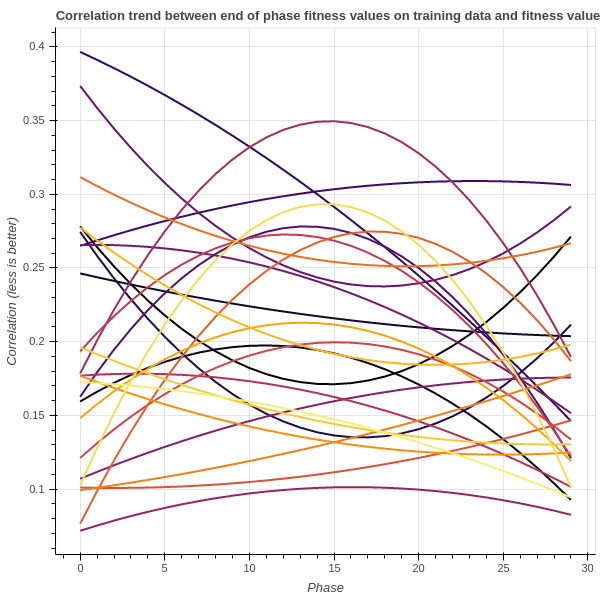
\includegraphics[width=0.8\linewidth]{figures/usecasecorrdisconnected.png}
        \caption{Correlation behavior without communication.}
    \end{subfigure}
    \begin{subfigure}{0.5\textwidth}
        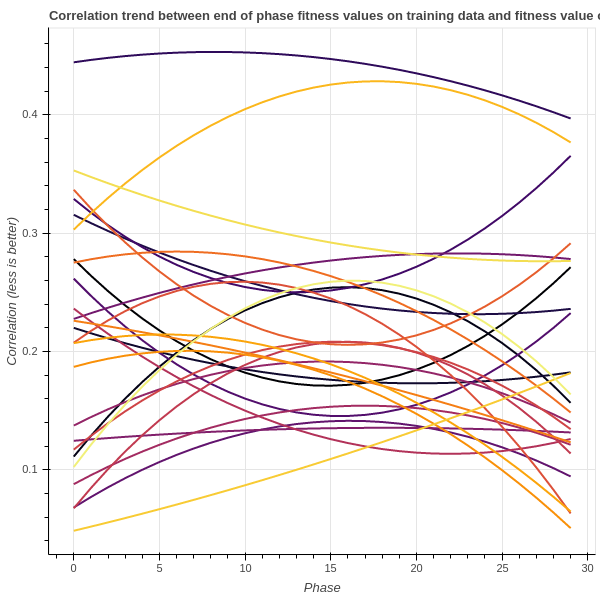
\includegraphics[width=0.8\linewidth]{figures/usecasecorrtree.png}
        \caption{Correlation behavior with tree topology.}
    \end{subfigure}
        \begin{subfigure}{0.5\textwidth}
        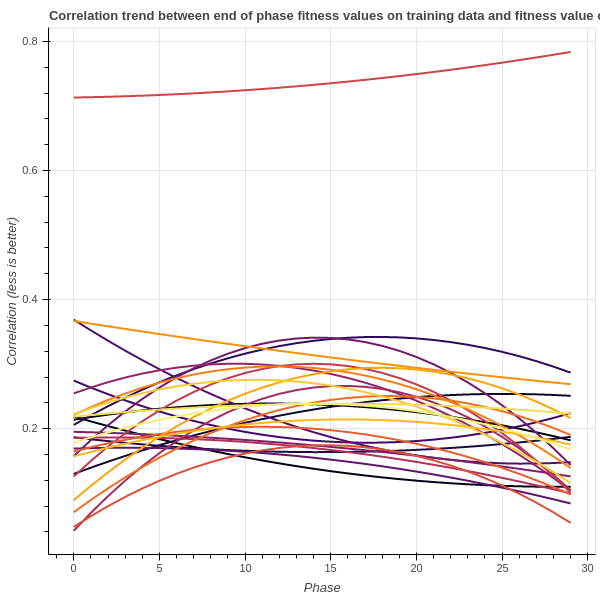
\includegraphics[width=0.8\linewidth]{figures/usecasecorrgrid.png}
        \caption{Correlation behavior with grid topology.}
    \end{subfigure}
    \begin{subfigure}{0.5\textwidth}
        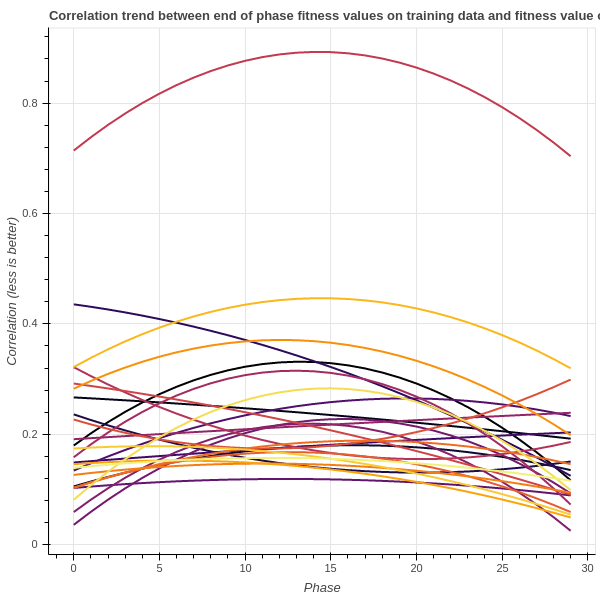
\includegraphics[width=0.8\linewidth]{figures/usecasecorrrandom.png}
        \caption{Correlation behavior with random topology.}
    \end{subfigure}
    \caption{Use case : Effect of topology on fitness correlation of distributed processes.}
    \label{fig:usecasecorrelation}
\end{figure}
In Figure \ref{fig:usecasecorrelation} we can clearly see how the topology affects the correlation between fitness values on training and validation data. Our validation configuration introduced in section \ref{KCV} promotes this behavior, the group of processes approximates k-fold cross validation. In a fully connected topology with minimal distance such as the grid, the correlation behavior will tend to the same value. We see a similar effect for the random topology. Note that this random topology consisted of disconnected cycles as seen in Figure \ref{fig:topologies}. The disconnected topology has  a near uniformly distributed correlation, there is no communication between the processes so they cannot train on the validation data. This is a parallel execution of 25 sequential processes with differing seeds and data. The tree topology finds the middle ground, as we descend toward the leaves the amount of shared information increases and with it the coverage of the validation data.
We can also see from the plots how the process evolves over time. The grid and random topology quickly stabilize without significant gain. The tree topology has a subset of processes that starts to converge to a lower correlation value. 

\subsection{Resulting Model}
We now look at the expression with the lowest fitness value for the validation data. This is after all the aim of the tool, returning to the practitioner a surrogate model with an optimal fit. In Figure \ref{fig:bestusecase} we see the resulting tree with depth 6. We select the best expression returned by the distributed application of CSRM with a tree topology, given its benefits in runtime and scaling. The distributed run is seeded by the 10/20/30 run. The resulting expression has a fitness value of 0.039 on the full data set. While this value is low, it is still 10 orders of magnitude removed from the optimal. This expression therefore represents an intermediate result and gives us an indication of the value partial results can offer.
\begin{figure}
    \centering
    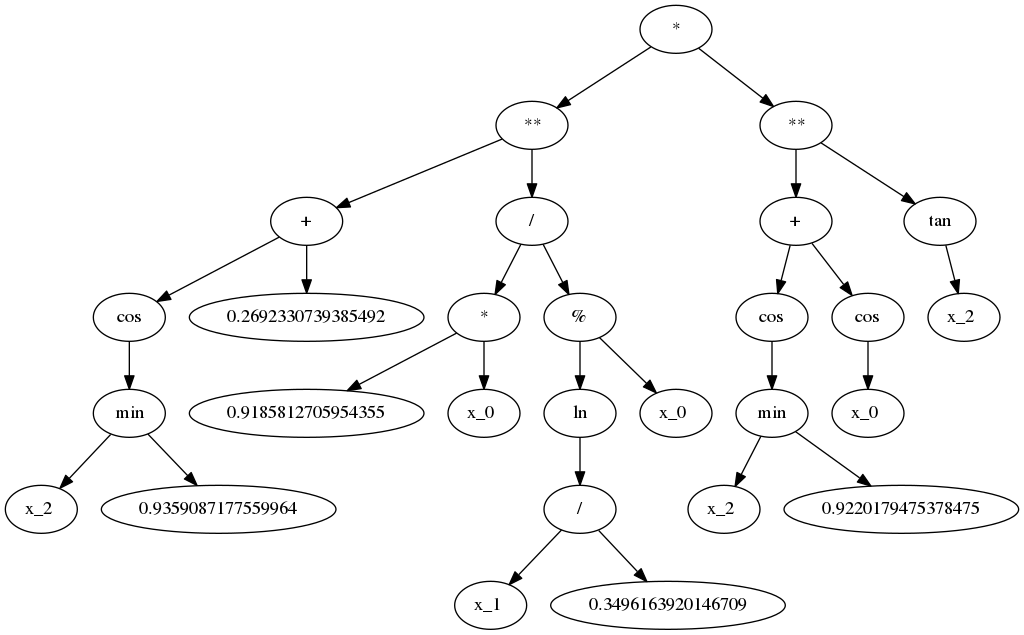
\includegraphics[width=\textwidth,height=\textheight,keepaspectratio]{figures/bestusecasesimple.png}
    \caption{Fittest expression for simulator use case.}
    \label{fig:bestusecase}
\end{figure}
\paragraph{Response plots}
While this model offers an analytical expression that we can evaluate, it is non trivial to conclude from this expression alone how the attack rate responds to variations in the three parameters. We use response plots for each parameter in order to isolate the effect each parameter has. We vary each of the parameters while keeping the other two constant. For the constant value we select the midpoint of the range. We then observe the effect on the attack rate. It is important to note that the range of the attack rate is [0,1]. 
\begin{figure}
    \begin{subfigure}{0.9\textwidth}
        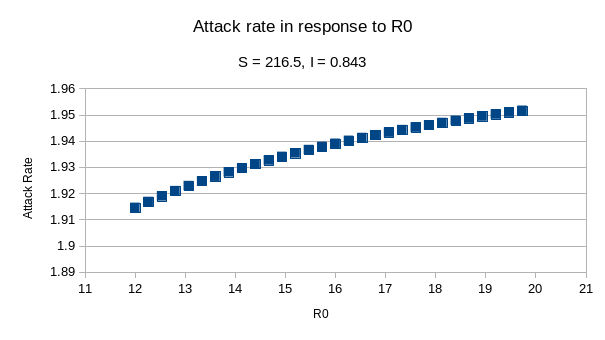
\includegraphics[width=0.8\linewidth]{figures/responseR.png}
        \caption{Response of attack rate to R.}
    \end{subfigure}
    \begin{subfigure}{0.9\textwidth}
        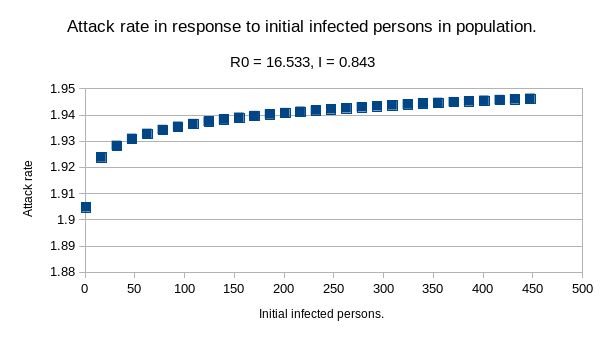
\includegraphics[width=0.8\linewidth]{figures/responseS.png}
        \caption{Response of attack rate to S.}
    \end{subfigure}
        \begin{subfigure}{0.9\textwidth}
        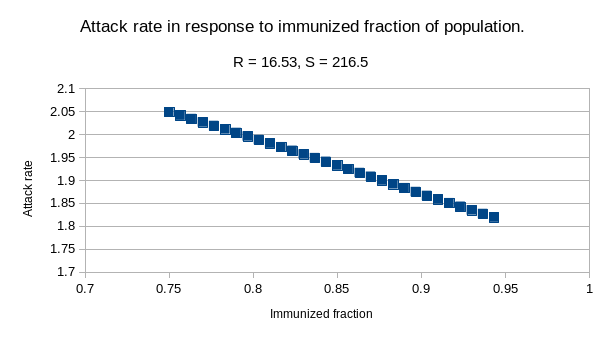
\includegraphics[width=0.8\linewidth]{figures/responseI.png}
        \caption{Response of attack rate to I.}
    \end{subfigure}
    \caption{Response plots of intermediate surrogate model.}
    \label{fig:usecaseresponseplots}
\end{figure}
We observe 2 important effects. First, our model produces an attack rate outside of the valid range of [0,1]. There is a scaling factor of 10 between the output of the model and the actual output data from the simulator. This is simply due to the fact that convergence is still in an intermediary phase. An important observation here is that our tool evolves the model based on 30 data points and not the full factorial design. This means that the response plots will use the model to evaluate points that are not necessarily available to our tool to train on. Second, the trend in the response plots is in line with what we expect to see in such a surrogate model. When R0 increases the attack rate increases, which is in line with theoretical and empirical results. A similar trend is visible with the initial number of infected persons, where R0 shows a logarithmic response. Finally, as the immunization fraction increases we see a negative linear response in the attack rate. We have chosen this suboptimal surrogate model to demonstrate that while the exact values of the attack rate are not yet correctly modelled, the expected trends are. This conclusion is vital to justify our incremental approach. We can see that surrogate models will focus on matching the trend first, rather than matching individual points. This is in part due to our usage of the Pearson R correlation coefficent as a basis for the fitness function. 



\subsection{Conclusion}
\paragraph{Results}
We have seen that incremental use of symbolic regression can, when applied judiciously, increase convergence compared to a blind search with the same computational cost. In addition to obtaining improved results we can integrate it with a simulator that produces output in parallel. 
The domain expert is ideally placed in order to select the sequence of configurations used in this incremental process. With domain specific information and experience the expert is well placed to select those configurations that are most likely to generate interesting new output patterns. Careful sequencing of the configurations is equally important in order to prevent a bias from being introduced in the process. A simple linear split as we have applied can, depending on the design and the parameter ranges, quite easily introduce such a bias.
As we have seen, the split in the data should be chosen carefully. Ideally one should aim for the same $\frac{4}{5}$ ratio of old/new data as is used in the training/validation ratio. If we apply this reasoning to the 30 point dataset, a reasonable split would be : 15/20/25/30. With small increments the risk for a bias is minimized. The first set of points is significantly larger than the increment itself, if the number of datapoints given to the SR tool is too small undesirable effects such as overfitting and constant aliasing are more likely to occur.
Applying the constant optimizers on seeded expressions demonstrated that overfitting is a real risk. This confirms our conclusion from section \ref{subsec:optimizers}.
In the distributed approach we observed that the grid topology offered the best fitness gains, at a severe cost in performance. The tree topology found the middle ground between performance and fitness improvement. The tree topology exploited the delay mechanism in order to obtain the best possible speedup.
We observed that our tool is capable of generating intermediary models that, even though suboptimal, demonstrate trends in their output that correlate strongly with the underlying model. This result suggests that the feedback loop between simulator, regression tool and domain expert can be valid even when only partial results are available. The time spent waiting on the simulator can now be used to obtain intermediary results that already offer insights into the underlying process.

